\documentclass{standalone}
\usepackage{tikzducks}

\begin{document}

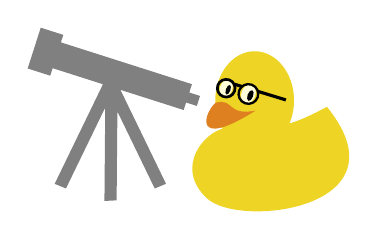
\begin{tikzpicture}
\duck[glasses];

\begin{scope}[scale=0.7,yshift=90,xshift=10]
	\fill[gray] (-2.9466,0.3003) -- (-3.1837,-0.4402) -- (-2.7744,-0.5708) -- (-2.7308,-0.4348) -- (-1.8176,-0.7262) -- (-2.6937,-2.5325) -- (-2.4891,-2.6173) -- (-1.7766,-1.1484) -- (-1.7910,-2.8438) -- (-1.5698,-2.8326) -- (-1.5560,-1.2208) -- (-0.8785,-2.6173) -- (-0.6739,-2.5325) -- (-1.5011,-0.8272) -- (-0.3532,-1.1935) -- (-0.3096,-1.0574) -- (-0.1147,-1.1196) -- (-0.0566,-0.9382) -- (-0.2516,-0.8760) -- (-0.2032,-0.7249) -- (-2.5809,0.0337) -- (-2.5373,0.1697) -- (-2.9466,0.3003) -- cycle;
\end{scope}
\end{tikzpicture}

\end{document}
